\documentclass[tikz,border=10pt]{standalone}
\begin{document}
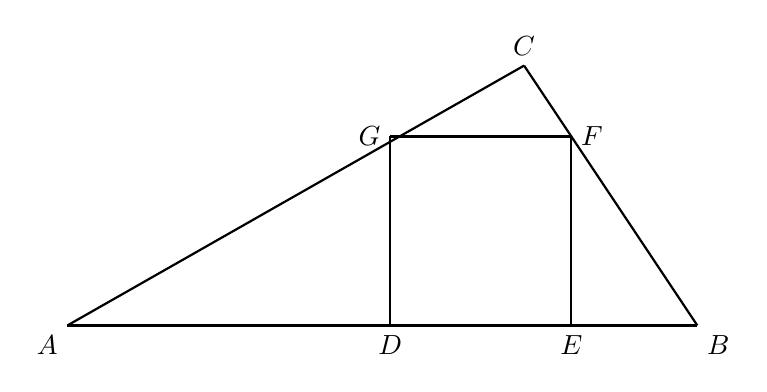
\begin{tikzpicture}[scale=1]
  \coordinate (A) at (0,0);
  \coordinate (B) at (8,0);
  \coordinate (D) at (4.1,0);
  \coordinate (E) at (6.4,0);
  \coordinate (G) at (4.1,2.4);
  \coordinate (F) at (6.4,2.4);
  \coordinate (C) at (5.8,3.3);

  \draw[thick] (A) -- (B);
  \draw[thick] (A) -- (C);
  \draw[thick] (C) -- (B);
  \draw[thick] (D) -- (G);
  \draw[thick] (G) -- (F);
  \draw[thick] (F) -- (E);

  \node[below left] at (A) {$A$};
  \node[below right] at (B) {$B$};
  \node[above] at (C) {$C$};
  \node[below] at (D) {$D$};
  \node[below] at (E) {$E$};
  \node[left] at (G) {$G$};
  \node[right] at (F) {$F$};
\end{tikzpicture}
\end{document}
